\chapter{Event Categorisation}
\label{chap:event_select}

\newpage
\section{Overview and Objectives}
Once a set of candidate photons is assembled we tag and categorise events using extra final-state objects characteristic of particular Higgs production modes.
The objective of this tagging procedure is to enhance overall signficance, to construct categories of events with superior mass resolution, and to separate out the Higgs production modes for individual measurement. 


The event categorisation begins with a selection on the photon candidates with $p_{T}^{\gamma1}/m_{\gamma\gamma} > 1/3$, $p_{T}^{\gamma2}/m_{\gamma\gamma} > 1/4$, and $100 < m_{\gamma\gamma} < 180$\,GeV.
The use of mass-scaled $p_{T}$ here and in later machine learning models serves a dual purpose: firstly it avoids distortion of lower values in the $m_{\gamma\gamma}$ spectrum, secondly it avoids introducing mass bias from the simulated data during model trainings. 
There are then further requirements on the photons' supercluster pseudorapidities: both must have $|\eta| < 2.5$ to keep them in the fiducial region of the ECAL, and also must not be in the barrel-endcap transition region $1.44 < |\eta| < 1.57$ to ensure full containment of the electromagnetic showers. 


\subsection{The Diphoton BDT}
Selected diphoton candidates are then evaluated for signal-like kinematics and mass resolution by a BDT, the diphoton BDT, whose output score is used as a discriminating variable by the tags.
The input features of this BDT are the following:
\begin{itemize}[leftmargin=.5in,noitemsep]
    \item The mass-scaled transverse momentum $p^{\gamma}_{T}/m_{\gamma\gamma}$ for the leading and subleading photons
    \item The pseudorapidity $\eta$ for the leading and subleading photons
    \item The cosine of the azimuthal angle $\Delta\phi$ between the photons
    \item The score from the photon identification BDT for both photons
    \item The mass resolution estimate given the assumption that the correct vertex is selected, $\sigma^{RV}_{\gamma\gamma}/m_{\gamma\gamma}$
    \item The mass resolution estimate given the assumption that the incorrect vertex is selected, $\sigma^{WV}_{\gamma\gamma}/m_{\gamma\gamma}$
    \item The probability that the correct diphoton vertex has been selected, $p^{RV}$, estimated with the vertex probability BDT
\end{itemize}

%The in the right-vertex case, diphoton mass resolution is estimated by propagating the individual photon energy resolution estimates.

In the right vertex case the mass resolution is assumed to be completely dominated by the ECAL photon energy resolution. 
These can be approximated by Gaussian distributions and combined in quadrature to give the following expression for mass resolution,
\begin{equation}
    \sigma^{RV}_{\gamma\gamma} = \frac{1}{2}\sqrt{(\sigma^{E}_{\gamma{1}}/E_{\gamma{1}})^2 + (\sigma^{E}_{\gamma{2}}/E_{\gamma{2}})^2}
\end{equation} 
where $\sigma^{E}_{\gamma{1}}/E_{\gamma{1}}, \sigma^{E}_{\gamma{2}}/E_{\gamma{2}}$ are the relative uncertainties on the photon energies for the leading and subleading photons respectively. 

(Wrong vertex case)
In the wrong vertex case an extra contribution to the mass resolution from the vertex is summed in quadrature with the expression for the right vertex case. 
\begin{equation}
    \sigma^{WV}_{\gamma\gamma} = \frac{1}{2}\sqrt{(\sigma^{RV}_{\gamma\gamma}/m_{\gamma\gamma})^2 + (\sigma^{V}_{\gamma\gamma}/m_{\gamma\gamma})^2}
\end{equation} 
The assumption of a Gaussian-distributed uncertainty here is justified in the following way 
(see Louie's thesis)


(Training)
The diphoton BDT is trained on background and all signal samples with some funny weighting. 
Weighted according to their SM cross sections and expected mass resolution (?)
\begin{equation}
    w^{sig} = \frac{p^{RV}}{\sigma^{RV}_{\gamma\gamma}/m_{\gamma\gamma}} + \frac{1-p^{RV}}{\sigma^{WV}_{\gamma\gamma}/m_{\gamma\gamma}}
\end{equation} 
Weighting examples during training can be considered to be like setting a priority for their correct classification. 
This weighting will prioritise the correct classification of high mass resolution events, and production modes with a larger cross section. 

The diphoton BDT is validated with \Zee events reconstructed as diphotons. The perfomance of the diphoton BDT is shown in figure X


Figure \ref{fig:event_categorisaton:diphoton_bdt} shows the diphoton BDT score distributions for SM signal and background samples and for the \Zee control region
\begin{figure}[h!]
    \begin{center}
        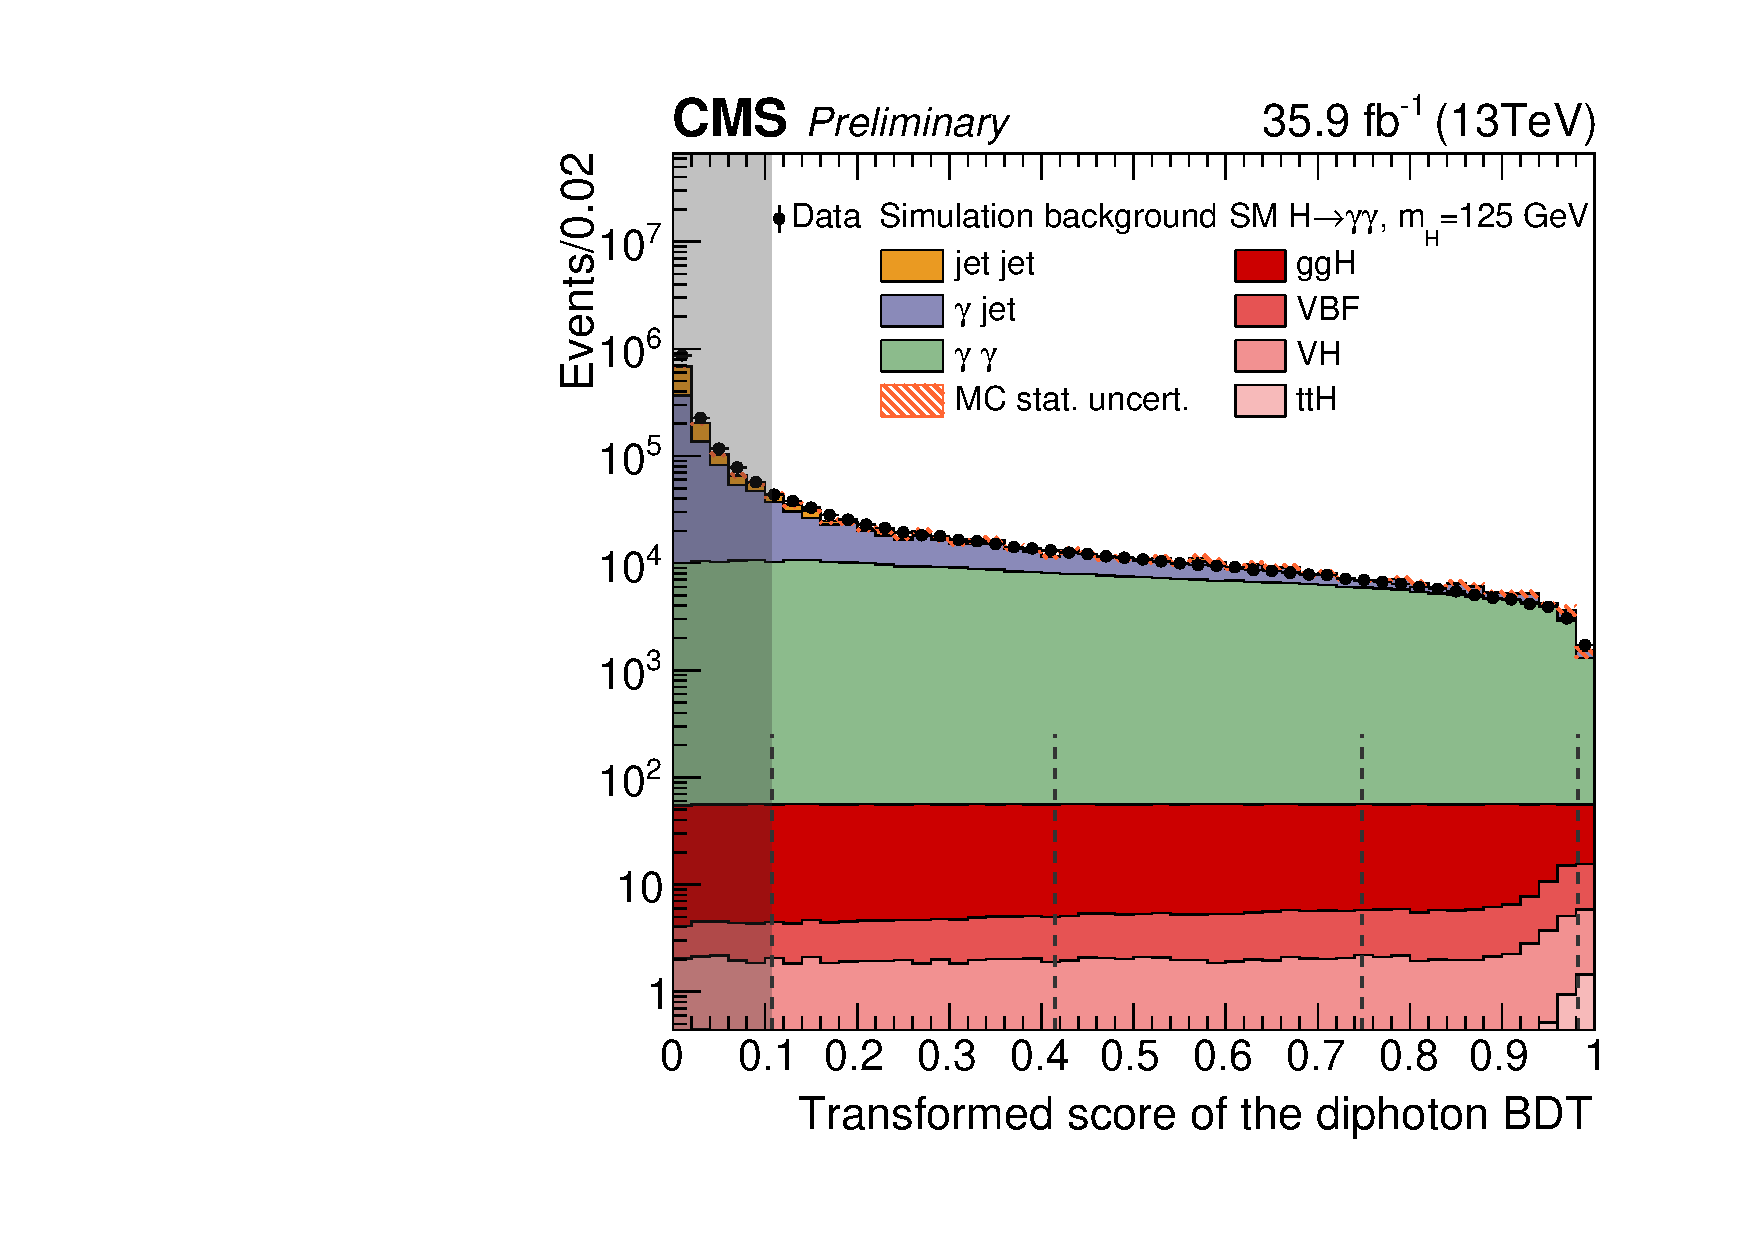
\includegraphics[width=0.49\textwidth]{figures/event_selection/Figure_005-a.pdf}
        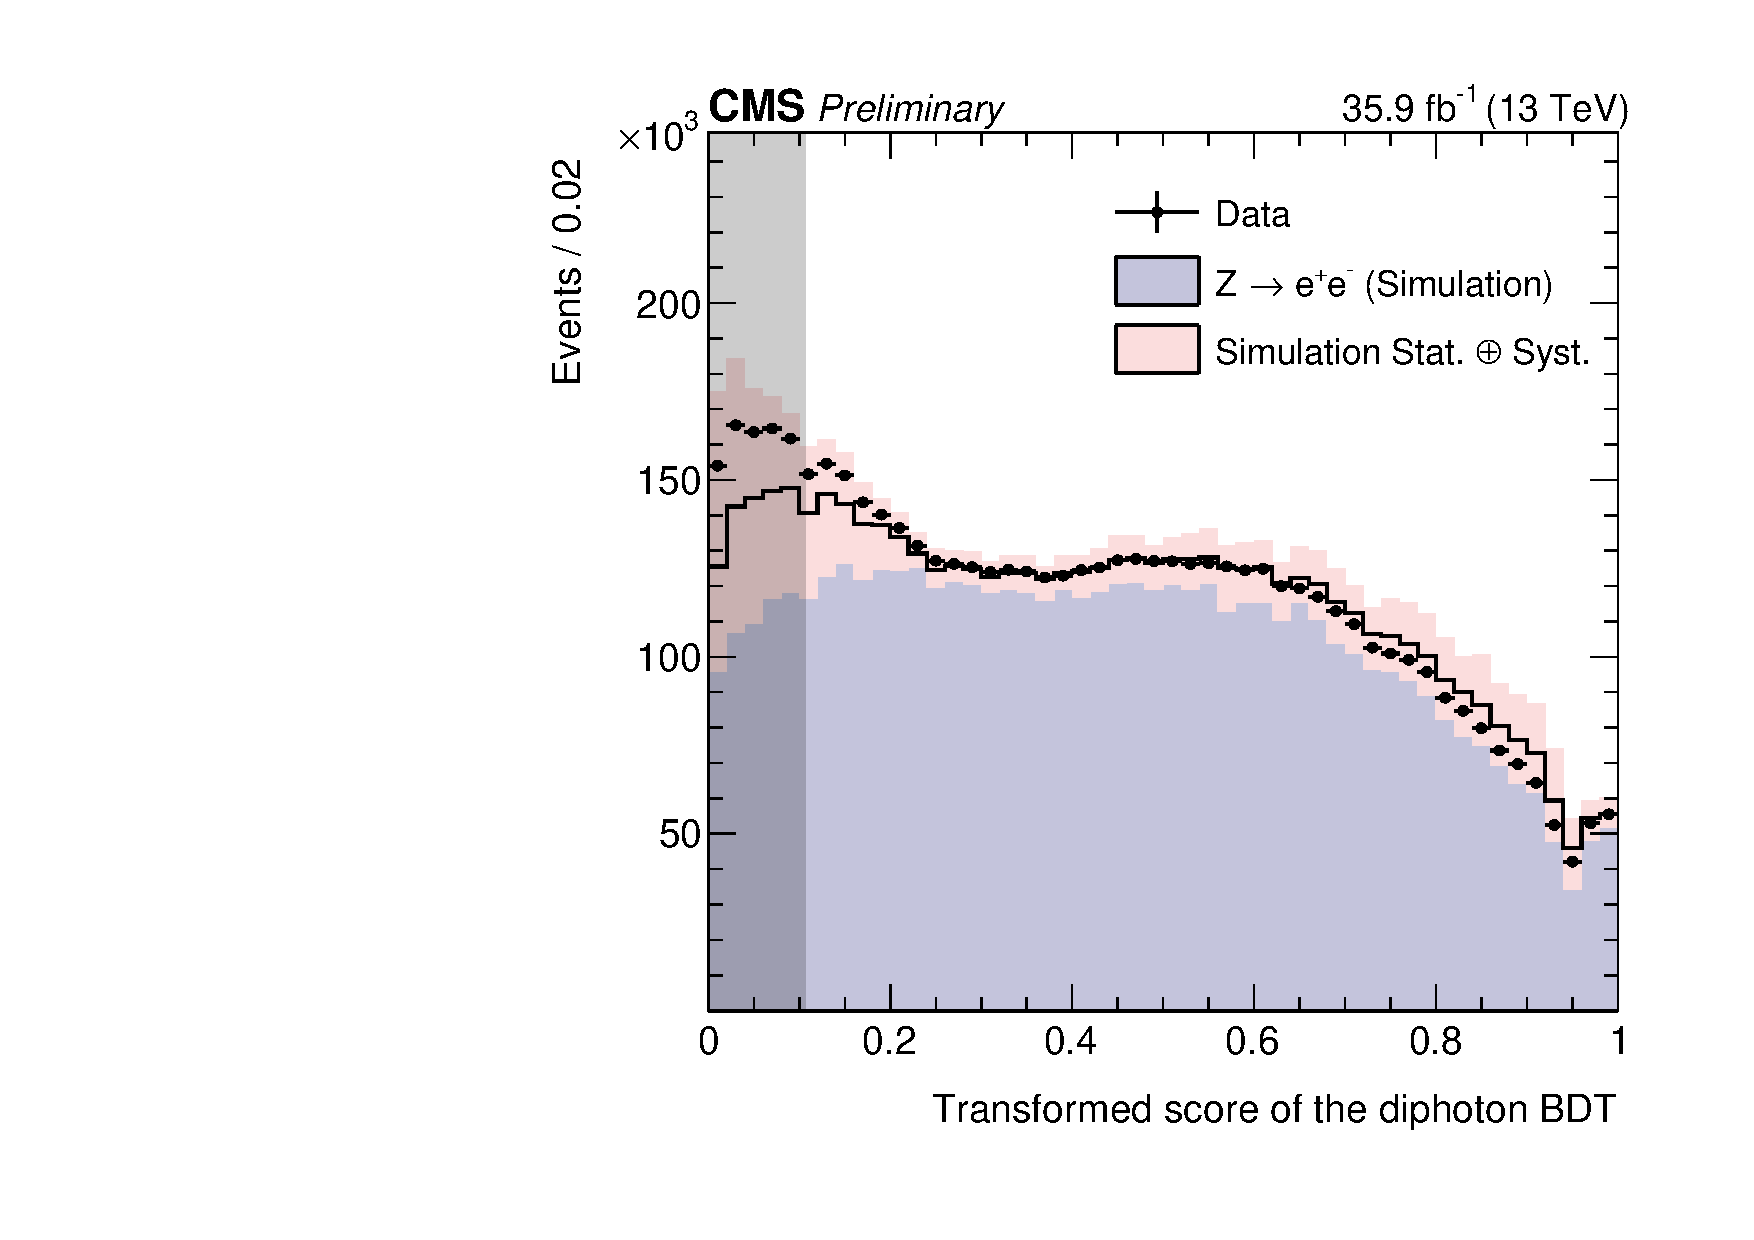
\includegraphics[width=0.49\textwidth]{figures/event_selection/Figure_005-b.pdf}
    \end{center}
    \caption{Crap figures with stupid flattened distributions}
        \label{fig:event_categorisaton:diphoton_bdt}
\end{figure}


\subsection{Tagging Scheme}
Tagging is implemented as a fall-through sequence where diphotons are offered to each tag in order of priority (Table \ref{tab:event_categorisaton:tag_sequence}). 
If a diphoton is not accepted by a tag it then passes to the next tag for consideration until the final `untagged' tag category. 
If the diphoton does not meet the criteria for this last tag it is discarded.
In the case of multiple tagged candidate diphotons in an event we select the one with the highest priority tag and category, if they are in the same category we choose the diphoton with the highest diphoton $p_{T}$.

\begin{table}[h!]
    \begin{tabular}{ l || l | l}
        Tag & Target Process & Structure \\
        \hline
        \ttH Leptonic      & \ttH with semi-leptonic top decays & Single category \\
        \ttH Hadronic      & \ttH with fully-hadronic top decays & Single category \\
        ZH Leptonic        & VH with leptonically-decaying Z boson & Single category \\
        WH Leptonic        & VH with leptonically-decaying W boson & Single category \\
        VH Leptonic Loose  & VH with leptonically-decaying W or Z boson & Single category \\
        VBF                & VBF with dijet in the final state & Three categories \\
        VH MET            & VH with significant amount of \MET & Single category \\
        VH Hadronic        & VH with hadronically-decaying W or Z boson & Single category \\
        Untagged           & Inclusive & Four categories \\
    \end{tabular}
    \caption{The \Hgg tag sequence}
    \label{tab:event_categorisaton:tag_sequence}
\end{table}

In the remainder of this chapter we will describe each tag grouped by the production mode they target. In particular we will consider VBF tagging in detail and present a tag based on jet images and a dense CNN. 






\section{Top Fusion Tagging}
In the \ttH production mode, a top-antitop pair is produced in association with the Higgs boson. The top quark immediately decays to a b quark and a W boson which will subsequently decay leptonically or hadronically. In the former (semi-leptonic) case there will be a bottom quark jet plus an associated lepton with \MET from the W decay. In the latter (fully-hadronic) case there will be a bottom quark jet plus two quark jets from the W decay to quarks (Figure \ref{fig:event_categorisaton:top_decays}). 

\begin{figure}[h!]
    \begin{center}
        \begin{tikzpicture}[baseline=(current bounding box.center)]
        \begin{feynman}
            \vertex (a) {$t$};
            \vertex [right=of a] (b);
            \vertex [above right=of b] (f1);
            \vertex [below right=of b] (f2) {$b$};
            \vertex [above right=of f1] (f3) {$q_{(u,c,t)}$};
            \vertex [below right=of f1] (f4) {$\bar{q}_{(d,s,b)}$};
            \diagram* {
                (a) -- [fermion] (b) -- [boson, edge label=\(W^{+}\)] (f1),
                (b) -- [fermion] (f2),
                (f1) -- [fermion] (f3),
                (f4) -- [fermion] (f1),
            };
        \end{feynman}
        \end{tikzpicture}
        %
        \qquad
        \begin{tikzpicture}[baseline=(current bounding box.center)]
        \begin{feynman}
            \vertex (a) {$t$};
            \vertex [right=of a] (b);
            \vertex [above right=of b] (f1);
            \vertex [below right=of b] (f2) {$b$};
            \vertex [above right=of f1] (f3) {$\bar{\ell}$};
            \vertex [below right=of f1] (f4) {${\nu_{\ell}}$};
            \diagram* {
                (a) -- [fermion] (b) -- [boson, edge label=\(W^{+}\)] (f1),
                (b) -- [fermion] (f2),
                (f1) -- [fermion] (f3),
                (f4) -- [fermion] (f1),
            };
        \end{feynman}
        \end{tikzpicture}
    \end{center}
    \caption{Top quark decay modes: a fully-hadronic decay (left) and a semi-leptonic decay (right).}
    \label{fig:event_categorisaton:top_decays}
\end{figure}

The top tags target these two decay modes: the leptonic tag searches for \ttH events where at least one top quark decays semi-leptonically, and the hadronic tag searches for \ttH events where both top quarks decay fully-hadronically. 

\subsection{\ttH Leptonic}
This tag uses a set of selections on kinematic properties of leptons and jets in the event. 
Leptons are required to pass selection requirements depending on their flavour
\begin{itemize}[leftmargin=.5in,noitemsep]
    \item Diphoton BDT score $> 0.11$ 
    \item At least one selected lepton with $p_{T} > 20$\,GeV
    \item All selected leptons are required to have an angular separation from a signal photon of $R(\ell,\gamma) > 0.35$
    \item $|m_{e\gamma} - m_{Z}| > 5$\,GeV (electrons only)
    \item A minimum of two jets in the event with $p_{T} > 25$\,GeV, $|\eta| < 2.4$, $R(j,\gamma) > 0.4$ and $R(j,\ell) > 0.4$
    \item At least one jet is tagged as b jet by the CSV tagger (medium requirement)
\end{itemize}


\subsection{\ttH Hadronic}
This tag uses a set of selections on kinematic properties of the jets in the event, as well as a dedicated BDT. The \ttH hadronic BDT is trained on the following input features:
\begin{itemize}[leftmargin=.5in,noitemsep]
    \item the number of jets with $p_{T} > 25$\,GeV,
    \item the $p_{T}$ of the leading jet,
    \item the two highest scores of the CSV b-tagger.
\end{itemize}
A selection on the BDT output score (Figure \ref{fig:event_categorisaton:tth_hadronic_bdt}) is optimised simultaneously on simulation with a selection on the diphoton BDT score to maximise expected precision on the signal strength of the \ttH production channel. 

\begin{figure}[h!]
    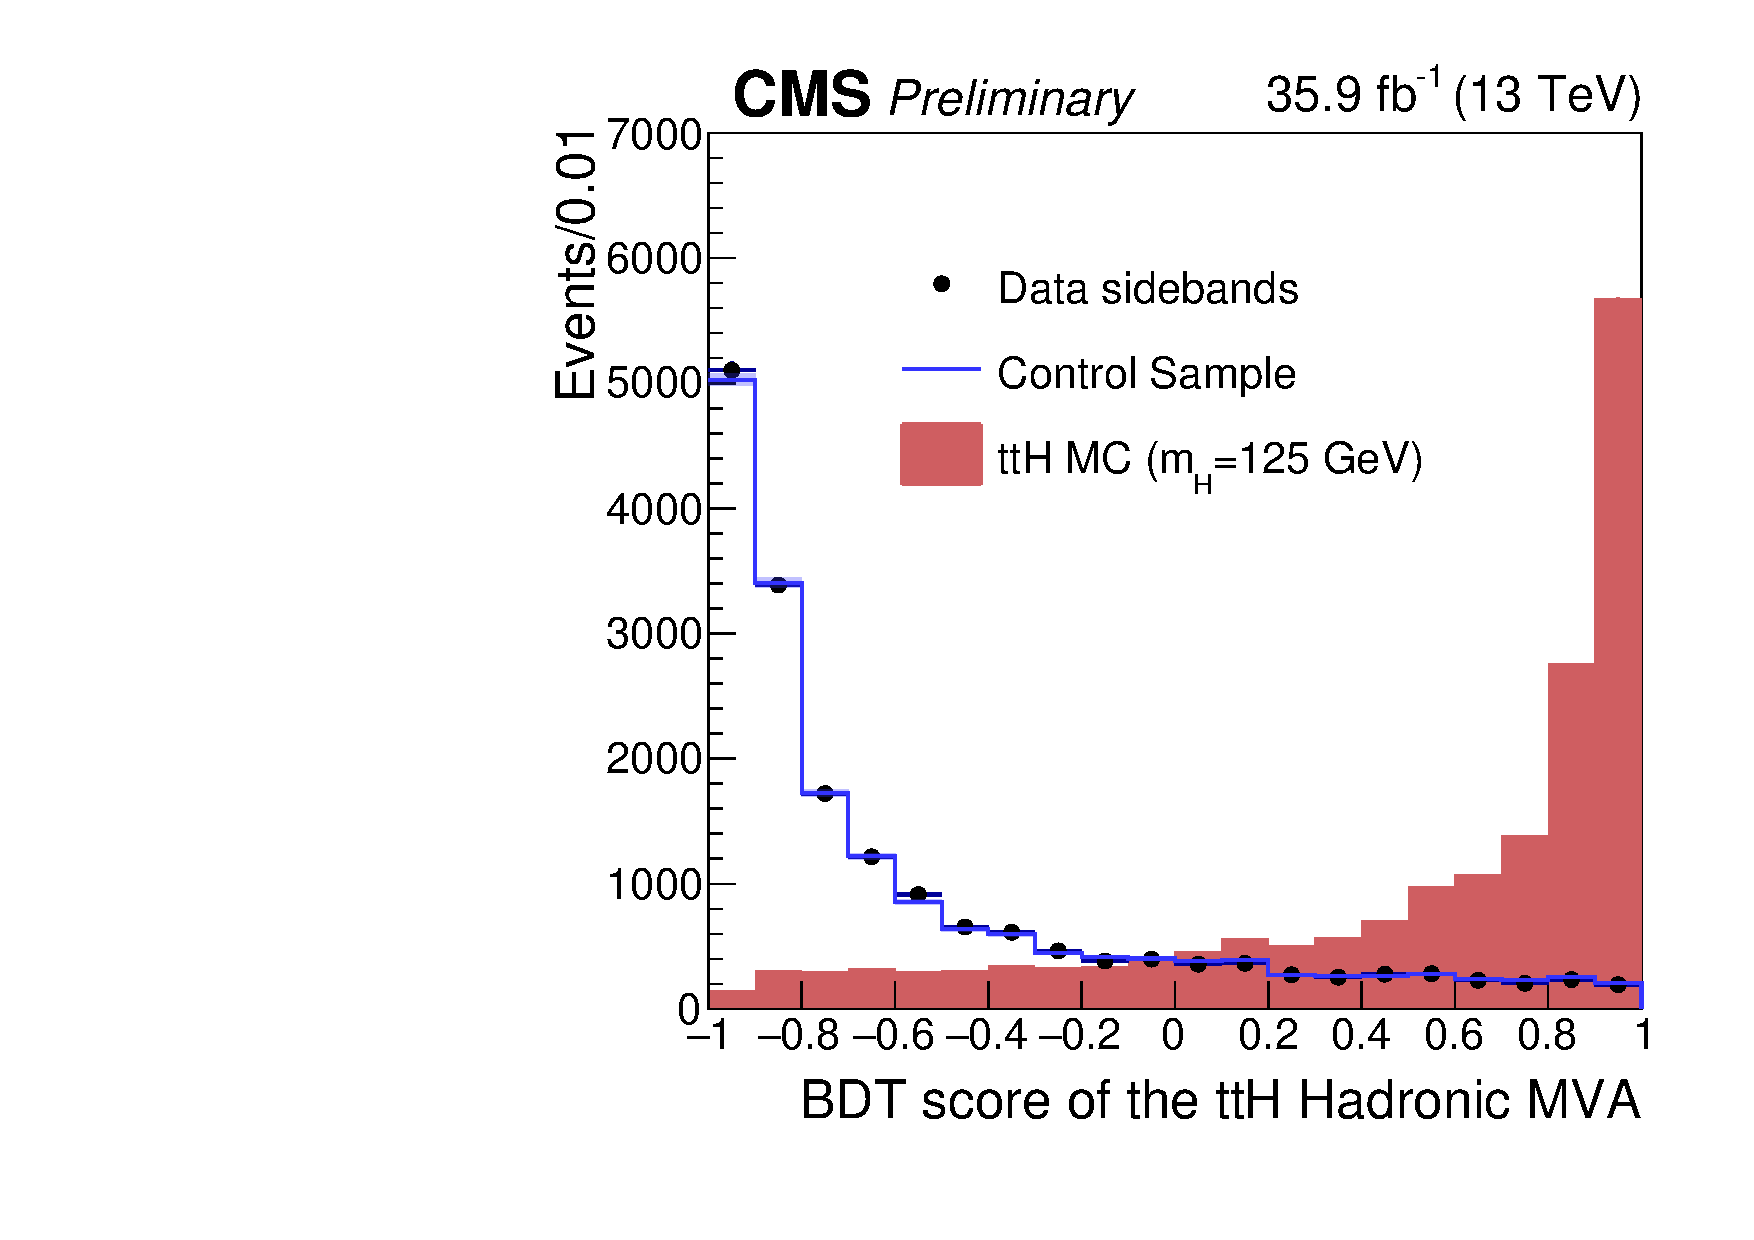
\includegraphics[width=0.49\textwidth]{figures/event_selection/Figure_006.pdf}
    \caption{Score distribution of the hadronic \ttH BDT. The blue lined histogram shows the distribution for the control region, the red filled histogram shows the score distribution for simulated signal, and the points show the score distribution of the data sideband regions ($m_{\gamma\gamma} < 115$\,GeV or $m_{\gamma\gamma} > 135$\,GeV).}
        \label{fig:event_categorisaton:tth_hadronic_bdt}
\end{figure}

A control region is constructed by selecting photon pairs where one passes the preselection and photon ID requirements, whilst the other has no preselection requirement and the photon ID is inverted.
These events are then weighted in $\eta$ and $p_T$ of the photons to reproduce the kinematic properties of the signal region.

The selection requirements of the \ttH Hadronic tag are as follows:
\begin{itemize}[leftmargin=.5in,noitemsep]
    \item $p_{T}/m_{\gamma\gamma} > 1/3$ and $1/4$ for leading and subleading photons respectively,
    \item diphoton BDT score $> 0.4$,
    \item no leptons that meet the criteria of the \ttH Leptonic tag
    \item a minimum of three jets in the event with $p_{T} > 25$\,GeV and $|\eta| < 2.4$,
    \item at least one jet is tagged as b jet by the CSV tagger (medium requirement),
    \item a \ttH Hadronic BDT score above 0.75.
\end{itemize}



\section{Associated Production Tagging}
In the associated production (VH) mode a W or Z is produced in association with the Higgs boson. The VH tags target different vector bosons decaying in different ways which can manifest as leptons, jets or \MET in the event.
All of the leptonic VH tags are selection-based and have various isolation requirements to avoid contamination from Drell-Yan background processes.

\subsection{ZH Leptonic}
Targets Higgs production in association with a Z boson that subsequently decays leptonically with stringent requirements. The selection criteria are as follows:
\begin{itemize}[leftmargin=.5in,noitemsep]
    \item $p_{T}/m_{\gamma\gamma} > 3/8$ and $1/4$ for leading and subleading photons respectively,
    \item diphoton BDT score $> 0.11$,
    \item two same-flavour leptons with $p_T > 20$\,GeV and satisfying the same requirements as in the \ttH Leptonic tag
    \item $70 < m_{\ell\ell} < 110$\,GeV,
    \item $R(\gamma,e) > 1.0$, or $R(\gamma,\mu) > 0.5$,
    \item conversion electron veto: if an electron and a photon share a supercluser, the electron track must be well-separated from the supercluser centre ($R(SC,e_{\mathrm{track}}) > 0.4$).
\end{itemize}


\subsection{WH Leptonic}
Targets Higgs production in association with a W$^{\pm}$ boson that subsequently decays leptonically with stringent requirements. The selection criteria are as follows:
\begin{itemize}[leftmargin=.5in,noitemsep]
    \item $p_{T}/m_{\gamma\gamma} > 3/8$ and $1/4$ for leading and subleading photons respectively,
    \item diphoton BDT score $> 0.28$,
    \item at minimum one lepton with $p_T > 20$\,GeV and satisfying the same requirements as in the \ttH Leptonic tag
    \item $R(\gamma,\ell) > 1.0$,
    \item \MET$> 45$\,GeV,
    \item a maximum of two jets each satisfying $p_T > 20$\,GeV, $|\eta| < 2.4$, $R(j,\ell) > 0.4$, $R(j,\gamma) > 0.4$,
    \item electron conversion veto as in the ZH Leptonic tag
\end{itemize}



\subsection{VH Leptonic Loose}
Targets Higgs production in association with either W$^{\pm}$ or Z which then decay leptonically. This tag uses a looser \MET selection of \MET$ < 45$\, GeV, with the rest of the selection being the same as WH Leptonic.

\subsection{VH MET}
Targets Higgs associated production with \MET from at least one missing lepton. The selection criteria are as follows:
\begin{itemize}[leftmargin=.5in,noitemsep]
    \item $p_{T}/m_{\gamma\gamma} > 3/8$ and $1/4$ for leading and subleading photons respectively,
    \item diphoton BDT score $> 0.79$,
    \item \MET$> 85$\,GeV,
    \item $|\Delta\phi(\gamma\gamma,E_{T}^{miss})| > 2.4$
\end{itemize}


\subsection{VH Hadronic}
Targets Higgs production in association with a W or Z boson that decays hadronically. The selection criteria are as follows:
\begin{itemize}[leftmargin=.5in,noitemsep]
    \item $p_{T}/m_{\gamma\gamma} > 1/2$ and $1/4$ for leading and subleading photons respectively, 
    \item diphoton BDT score $> 0.79$,
    \item a minimum of two jets with $p_T > 40$\,GeV and $|\eta| < 2.4$, $R(j,\gamma) > 0.4$,
    \item dijet invariant mass $60 < m_{jj} < 120$\,GeV,
    \item $|\mathrm{cos}{\theta^{*}}|$
\end{itemize}









\section{VBF Tag: Legacy}
The VBF production mode is characterised by its distinctive event topology and kinematics: two high-$p_{T}$ jets with large pseudorapidity separation. Furthermore, the dijet substructure will also be distinctive with both jets originating from quarks and having colour connection to the proton remnant. 

Other production modes can also produce a Higgs boson in association with jets. In particular, ggH can be a significant source of false positives due to its larger cross section and capacity to produce jets in next-to-leading order processes and from initial-state radiation at leading order. 

VBF tagging targets the VBF production mode by exploiting the distinctive properties of VBF dijets. In this section we will explore two approaches:
\begin{itemize}[leftmargin=.5in,noitemsep]
    \item A tag based on two BDTs with engineered kinematic features. This is the approach used in the 2016 \Hgg analysis. 
    \item A tag based on a single dense convolutional neural network that receives jet structure information in the form of images in addition to engineered kinematic features. 
\end{itemize}
Both tags use the same event preselection, and produce scores used to define event categories which enhance the expected significance of the VBF channel. 
The measure of significance used here is the approximate mean significance (AMS) which was introduced in the Higgs ML challenge (ref),
\begin{equation}
    \mathrm{AMS}_{2} = \sqrt{2\left( (s+b+b_{\mathrm{reg}})\log\left(1 + \frac{s}{b+b_{\mathrm{reg}}}\right) - s \right)}.
\end{equation}
Where $s$ is the total number of signal events, $b$ is the total number of background events, and $b_{\mathrm{reg}}$ is a regularisation term that reduces sensitivity to local optima due to spiky distributions. 

The legacy tag consists of two BDTs chained together which integrate different information to form a discriminant score. 
The first of these, the djiet BDT, evaluates how signal-like the events are based on kinematic information from the dijet and its relationship with the diphoton. 
The second BDT, the combined BDT, integrates information from multiple sources to produce the final discriminant score for classification. 

\subsection{Selection}

\subsubsection{Jet Selection}
Selection criteria are applied to individiual jets in addition to those described in the previous chapter before being considered for making the dijet. 
(The selections on the individual jets)
(PUJID because AMS value, mention Zee $\eta$ agreement stuff)




\subsubsection{Dijet Selection}
Dijets are formed by selecting the two highest-$p_T$ jets in the event which pass the jet selection requirements. If there are fewer than two jets the event is rejected by the VBF tag and falls through to untagged. 
Candidate dijets are required to meet the following selection:
\begin{itemize}[leftmargin=.5in,noitemsep]
    \item $p_{T}/m_{\gamma\gamma} > 1/3$ and $1/4$ for leading and subleading photon respectively,
    \item photon ID BDT score $> -0.2$ for both photons,
    \item dijet invariant mass $m_{jj} > 250$\,GeV,
    \item jet $p_{T} > 40$\,GeV and $> 30$\,GeV for the leading and subleading jets respectively,
    \item absolute pseudorapidity $|\eta| < 4.7$ for both jets.
\end{itemize}

The photon ID score requirement is due to the diphoton BDT assigning a high score to background diphotons which have a low photon ID score.
This is occuring becuase the diphoton BDT is trained over multiple signal processes with a cross-section weighting, this in turn leads to it to prioritise the accurate classification of ggH-like events where a diphoton is produced without associated objects. 
Signal events in the VBF phase space have a lower weighting and therefore the diphoton BDT does not separate these with the same level of priority. 
A strong indicator of ggH signal is that the diphoton has high $p_T$. The BDT appears to be allowing high-$p_T$ background events through without applying photon ID requirements. The photon ID cut of the VBF tag is aimed at reducing this effect. 







\subsection{Dijet BDT}
BDT that targets signal-like dijet kinematics. Receives the following features which are unbiased with respect to mass by construction:
\begin{itemize}[leftmargin=.5in,noitemsep]
    \item $p_{T}/m_{\gamma\gamma}$ for the leading and subleading photons
    \item $p_{T}^{j1}$ and $p_{T}^{j2}$, the transverse momenta of the leading and subleading jets respectively
    \item $m_{jj}$ the invariant mass of the dijet
    \item $\Delta\eta$ the pseudorapidity gap between the two jets
    \item $\mathrm{min}\Delta{R}(\gamma,j)$ the smallest angular separation between either of the diphoton photons and either of the dijet jets
    \item $|\Delta\phi_{\gamma\gamma{jj}}|$ the absolute azimuthal angular difference between the diphoton and dijet
    \item $|\Delta\phi_{jj}|$ the absolute azimuthal angular difference between the jets of the dijet
    \item $C_{\gamma\gamma}$ the diphoton centrality expressed as:
        \begin{equation}
            C_{\gamma\gamma} = \mathrm{exp}\left(-\frac{4}{(\eta_{j1} - \eta_{j2})^{2}}\left( \eta_{\gamma\gamma} - \frac{\eta_{j1} + \eta_{j2}}{2} \right)^{2}\right)
        \end{equation}
\end{itemize}




\begin{figure}[h!]
    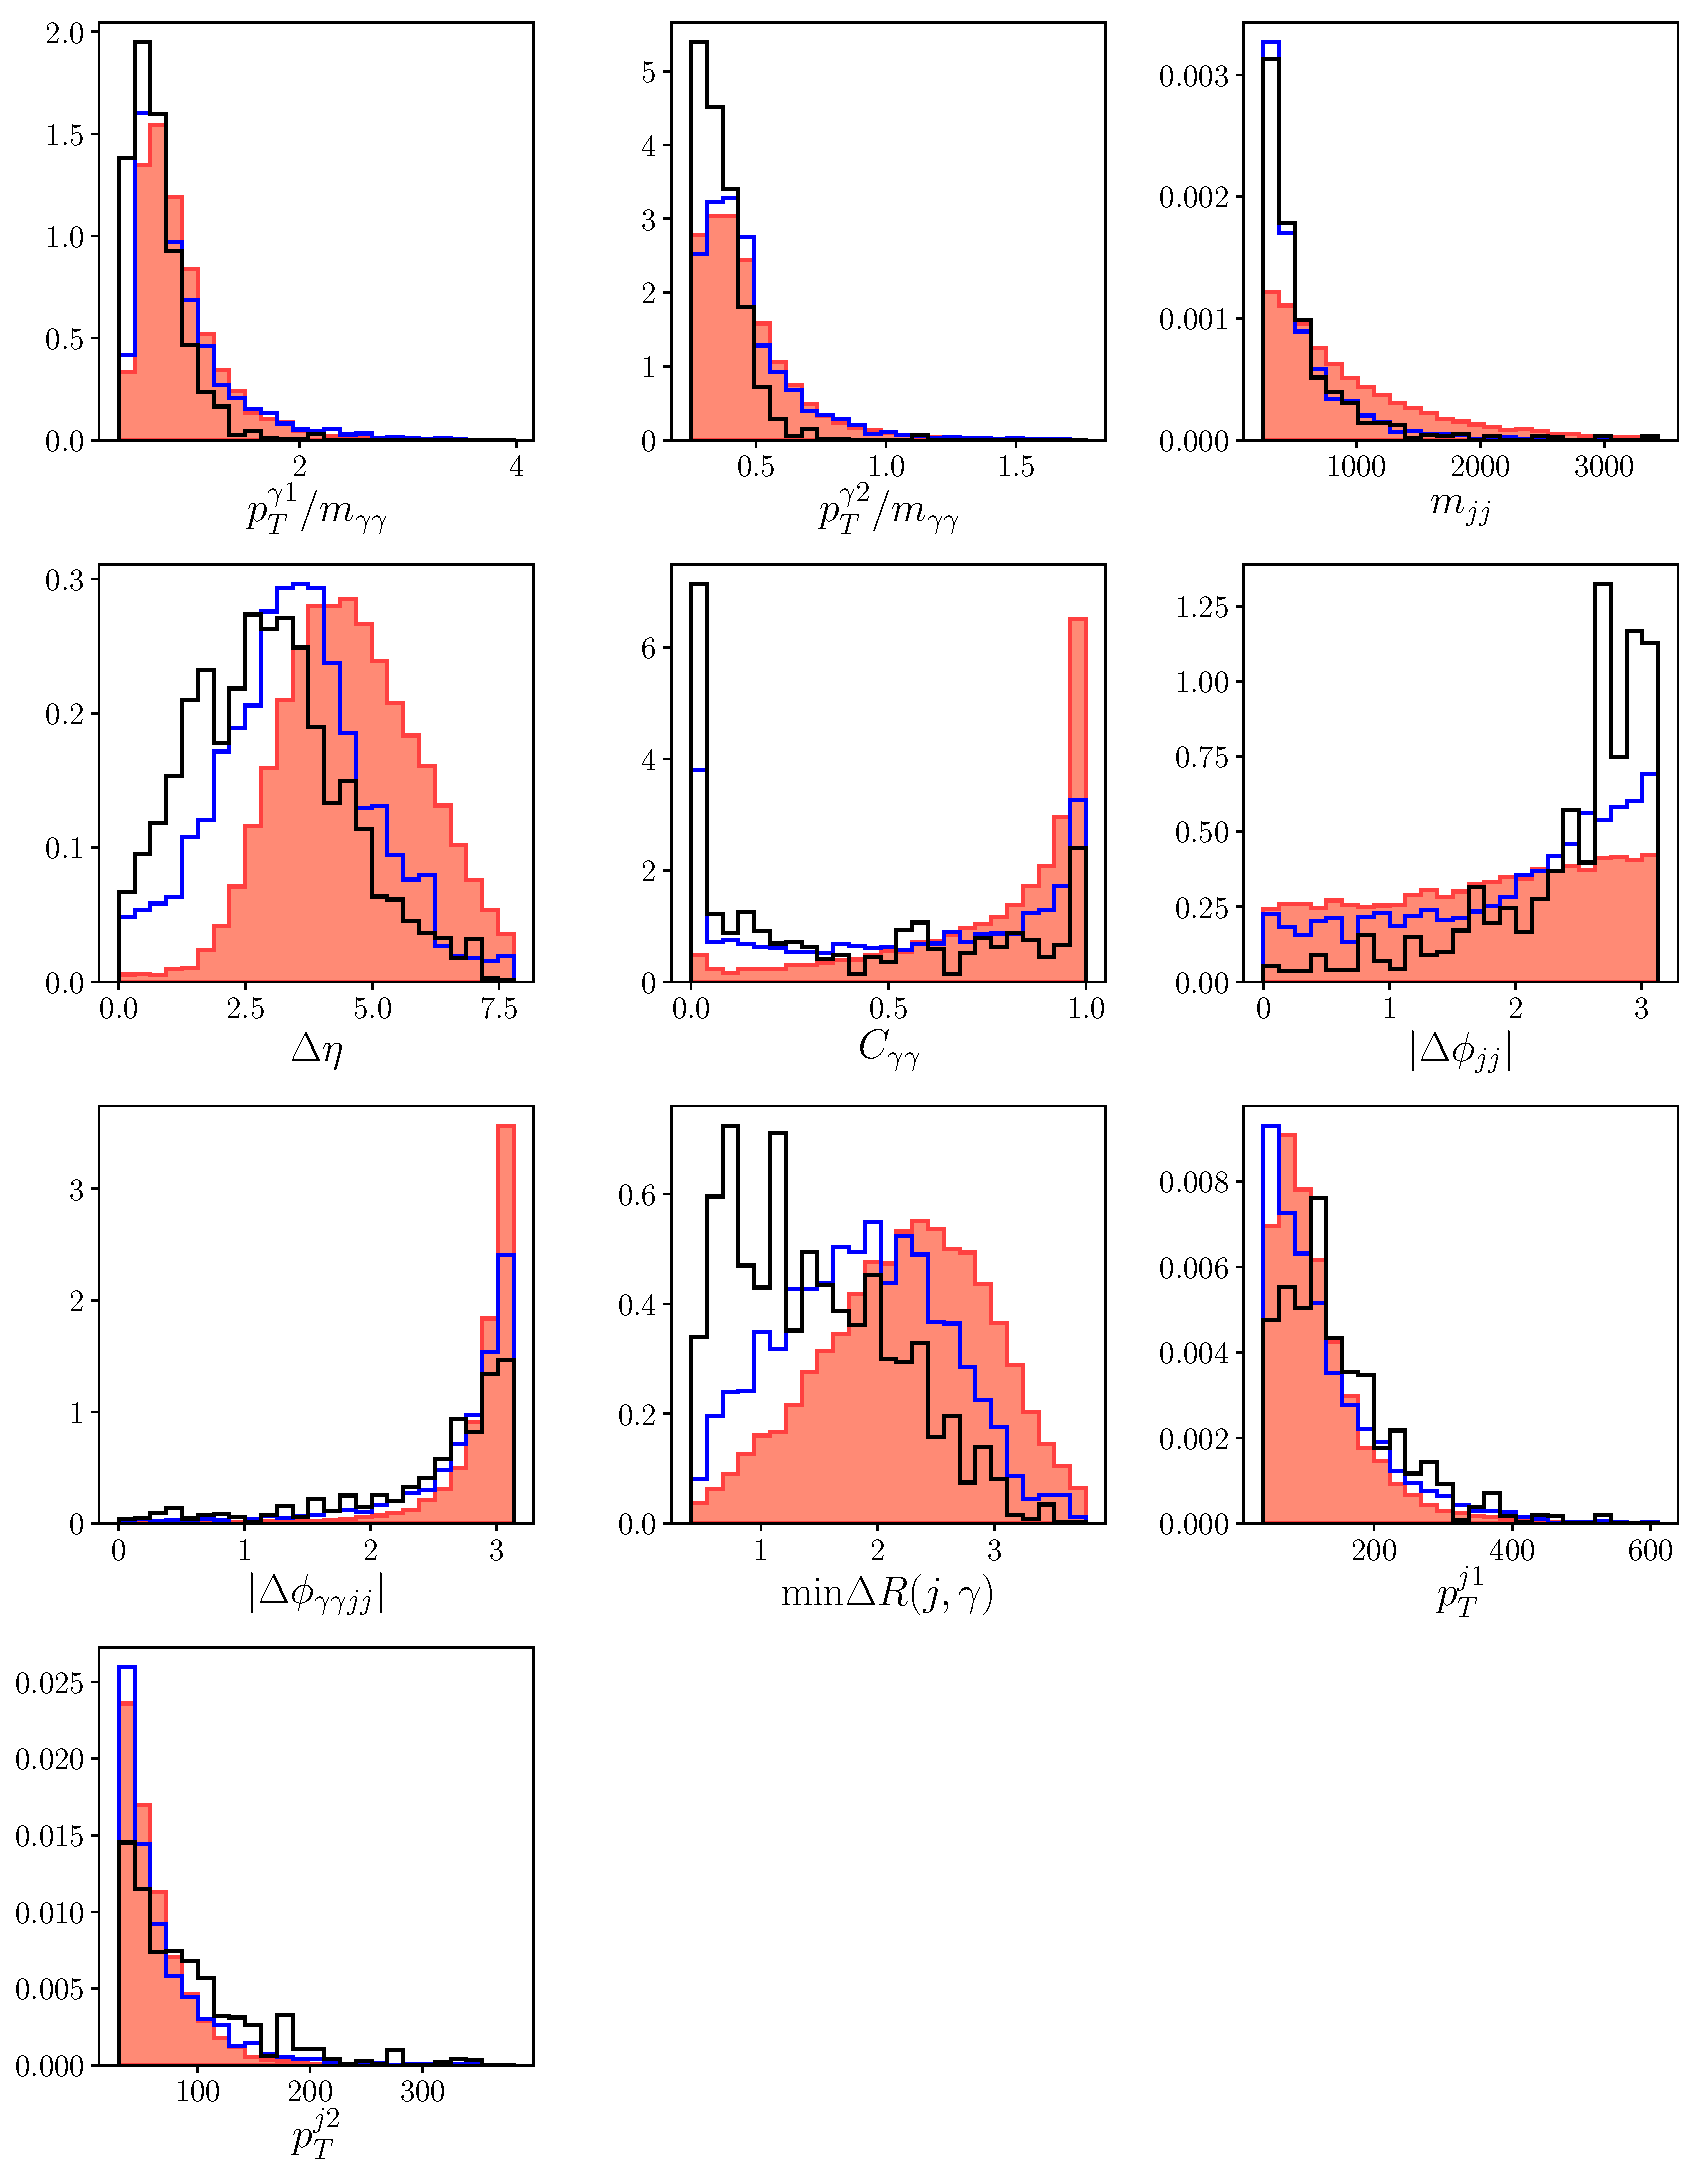
\includegraphics[width=0.90\textwidth]{figures/event_selection/dijet_BDT_features_PS.pdf}
    \caption{Dijet BDT feature distributions with the full VBF preselection. Distributions are all normalised to unity with solid red corresponding to VBF, blue line to ggH, and black line to SM background}
    \label{fig:event_categorisaton:dijet_bdt_features}
\end{figure}


\subsection{Combined BDT}
BDT that takes all the information and gives the final score
\begin{itemize}[leftmargin=.5in,noitemsep]
    \item diphoton BDT score
    \item dijet BDT score
    \item $p_{T}^{\gamma\gamma}/m_{\gamma\gamma}$, the mass-scaled transverse momentum of the diphoton
\end{itemize}

\begin{figure}[h!]
    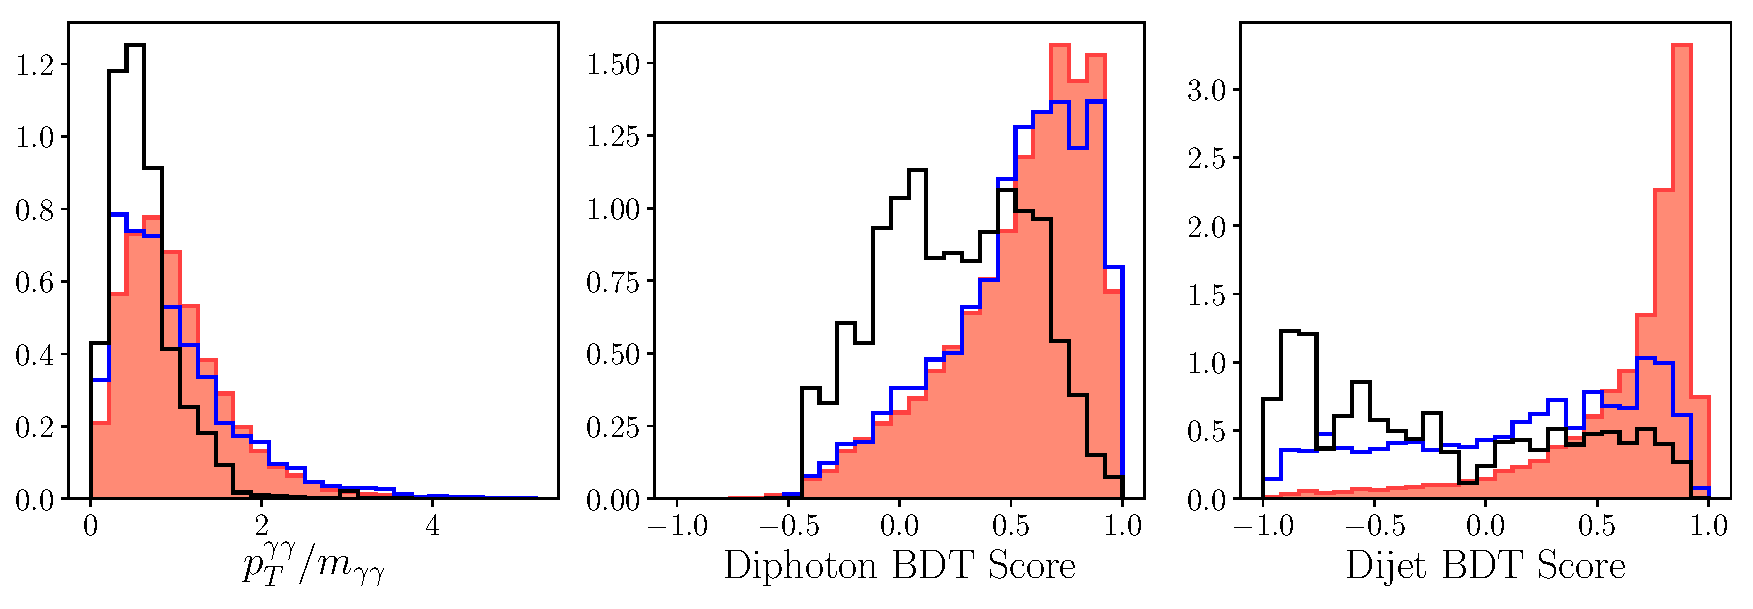
\includegraphics[width=0.90\textwidth]{figures/event_selection/combined_BDT_features_PS.pdf}
    \caption{Combined BDT feature distributions with the full VBF preselection. Distributions are all normalised to unity with solid red corresponding to VBF, blue line to ggH, and black line to SM background}
    \label{fig:event_categorisaton:combined_bdt_features}
\end{figure}

\begin{figure}[h!]
    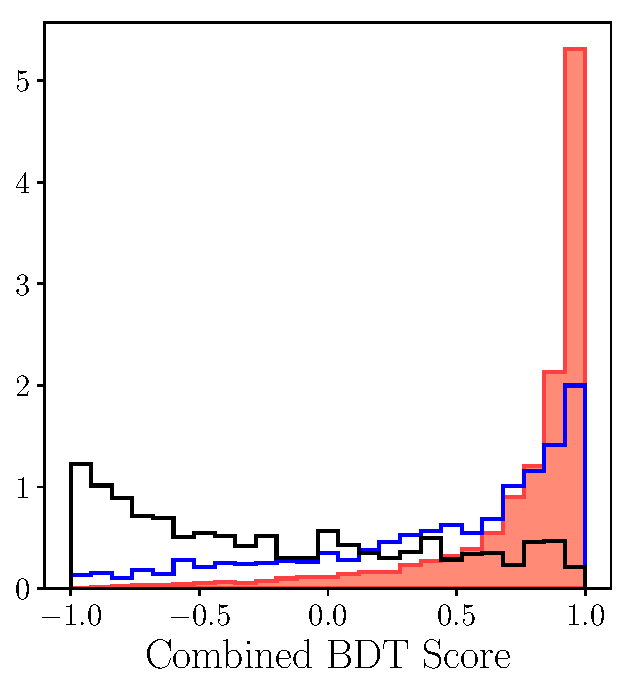
\includegraphics[width=0.4\textwidth]{figures/event_selection/combined_BDT_score.pdf}
    \caption{Combined BDT score distribution with the full VBF preselection. Distributions are all normalised to unity with solid red corresponding to VBF, blue line to ggH, and black line to SM background}
    \label{fig:event_categorisaton:combined_bdt_features}
\end{figure}





\subsection{Categorisation}
Boundary opt for overall significance


\subsection{Validation}
We define a control region in \Zee events where the electron veto has been inverted and the electrons reconstructed as photons. In addition to the electrons we require two jets with the following selection which mimics the phase space of the VBF tag:

\begin{itemize}[leftmargin=.5in,noitemsep]
    \item $p_{T}^{j1} > 40$, and $p_{T}^{j1} > 30$ for the leading and subleading jets,
    \item $p_{T}^{\gamma{1}} > 1/3$ and $p_{T}^{\gamma{2}} > 1/4$ for the leading and subleading photons.
\end{itemize}
There is no requirement on the dijet mass $m_{jj}$. 

The control region is used for simulation/data comparison of both the features input to the BDTs and the output scores. 

\begin{figure}[h!]
    \begin{center}
        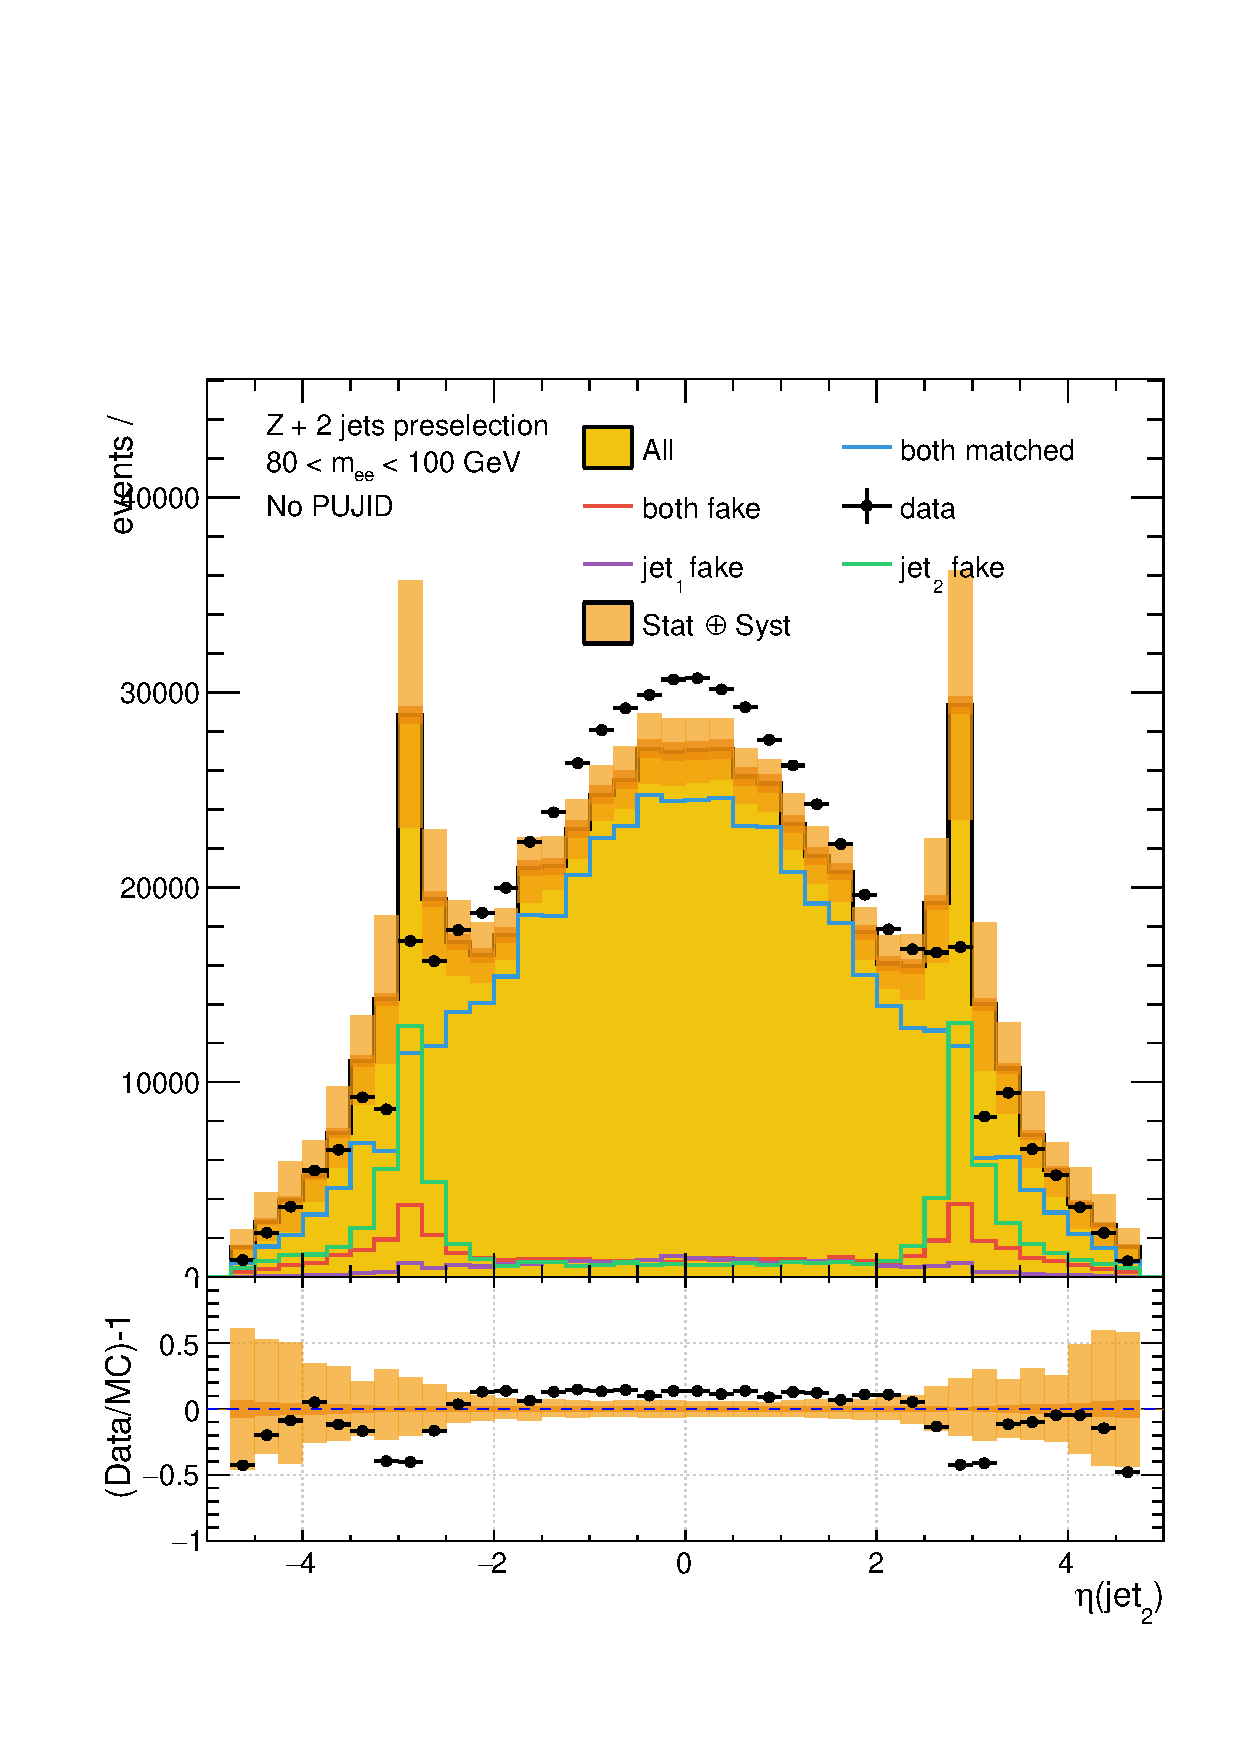
\includegraphics[width=0.45\textwidth]{figures/event_selection/stack_histogram_dijet_subleadEta_zplus2j_none_inclusive_.pdf}
        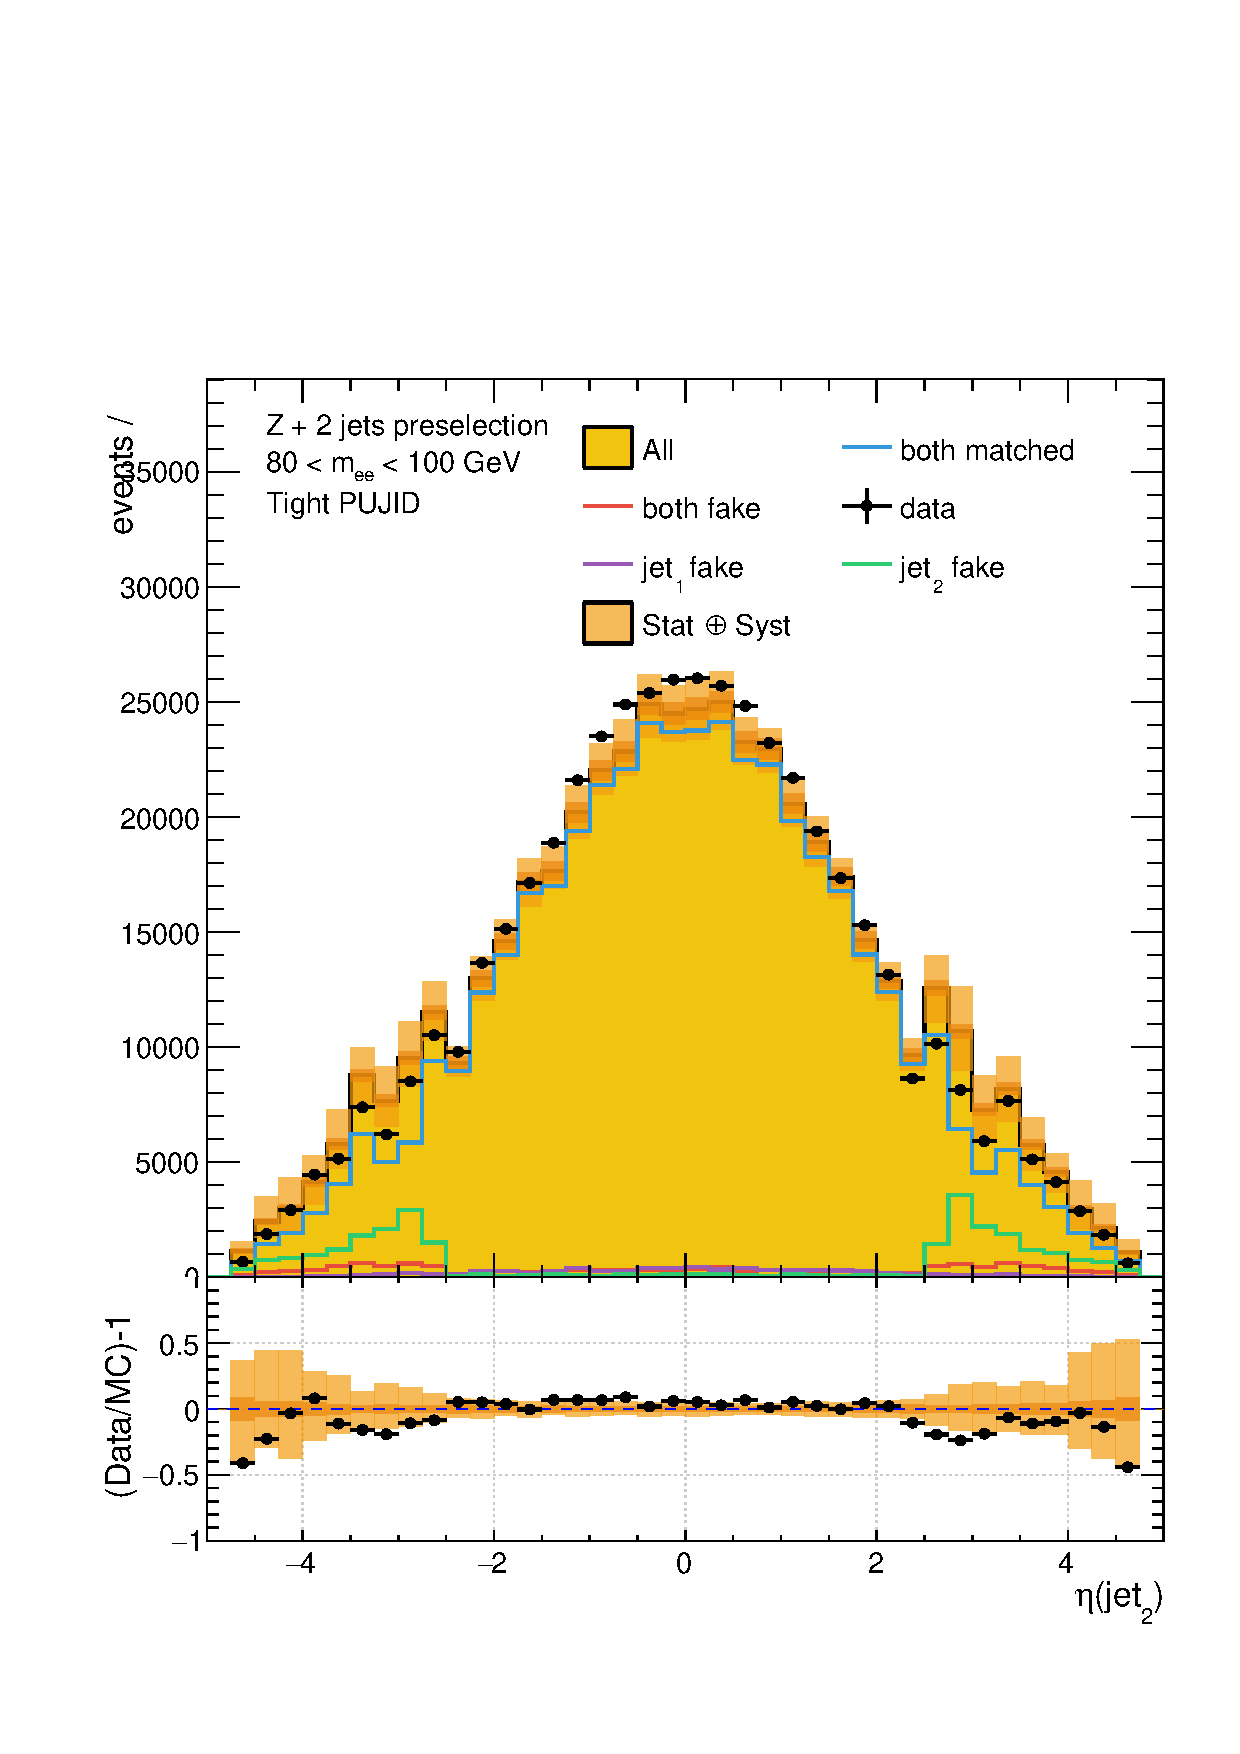
\includegraphics[width=0.45\textwidth]{figures/event_selection/stack_histogram_dijet_subleadEta_zplus2j_tight_inclusive_.pdf}
    \end{center}
    \caption{Sublead pseudorapidity for no PUJID and the tight working point. We note a substantial decrease in fake jets from the endcap/hadronic forward transition region around $|\eta|=3$, and an overall improvement in agreement between simulation and data.}
    \label{fig:event_categorisaton:sublead_eta_pujid}
\end{figure}








\section{VBF Tag: Dense Convolutional Neural Network}
Introduction, mention that the selection is the same, objectives and motivation for the new tag
The objective of the new tag is to use jet images and a dense CNN to enhance VBF signal extraction, especially VBF vs Gluon Fusion discrimination. 


\subsection{Jet Images}
The spatial distribution and properties of a jet's constituent particles contain important discriminating information about the originating parton. 
An image is a natural way of representing this information with the spatial distribution represented by the arrangement of pixel values and the channels of the image representing properties such as charged particle $p_{T}$ in the pixel region.

The image formulation used in this thesis is of two three-channel images stacked in the channels dimension to produce a $n\times{}n\times{}6$ dijet image.
The three channels are the following: $p_T$ deposition of charged candidates, $p_T$ deposition of neutral candidates, and particle multiplicity.
The space that the pixels correspond to is the space of particle displacements in pseudorapidity and azimuthal angle from the jet axis $(\Delta\eta,\Delta\phi)$,
\begin{equation}
    \begin{split}
        \Delta\eta =& \eta_{p} - \eta_{j} \\ 
        \Delta\phi =& \phi_{p} - \phi_{j} \\
    \end{split}
    \label{eq:event_categorisation:pixel_coords}
\end{equation}
where subscript $p$ denotes a constituent particle and $j$ denotes the jet. 
The pixels themselves are not a recilinear grid in $(\Delta\eta,\Delta\phi)$, but are evenly-spaced in the polar coordinates 
\begin{equation}
    \begin{split}
        \Delta{R} =& \sqrt{\Delta\eta^2 + \Delta\phi^2} \\
        \varphi   =& \mathrm{tan}(\Delta\phi/\Delta\eta) \\
    \end{split}
    \label{eq:event_categorisation:pixel_coords}
\end{equation}
These have been rotated by half a pixel in $\varphi$ so that the $(\Delta\eta,\Delta\phi)$ axes line up with the centres of a row of pixels rather than the boundary between them. 
Finally, the images are normalised such that the sum of the $p_T$-based channels equal one, and the sum of the individual multiplicity channels equal one. 
The image formulation is summarised in Figure \ref{fig:event_categorisation:jet_image}.

These images are different in their formulation and behaviour compared to a typical images.
Firstly, they are sparse with only a fraction of the pixels ever active in any one image. 
Secondly, assumptions about local correlations between pixels do not apply: two adjacent red pixels would mean two adjacent particles. Max pooling will simply pick the higher valued pixel during downsampling and information about the second particle will be lost. 
Thirdly, in the rectilinear image which is seen by the network (bottom right of Figure \ref{fig:event_categorisation:jet_image}) there is a periodic boundary condition where the top pixels wrap around to the bottom ones. When convolution operations are performed on these images the padding must be periodic in the vertical direction ($\varphi$ direction).






\newpage
\begin{figure}[h!]
    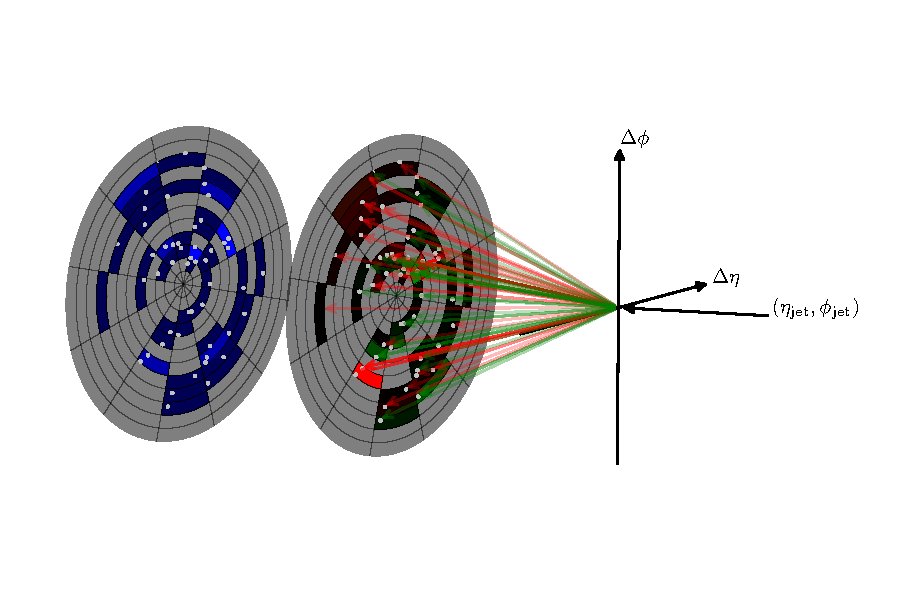
\includegraphics[width=\textwidth]{figures/event_selection/jet_diagram_RGB.pdf}
    \begin{center}
        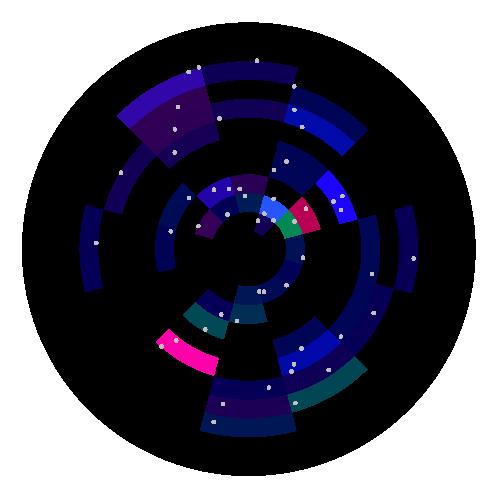
\includegraphics[width=0.49\textwidth]{figures/event_selection/full_image_polar.pdf}
        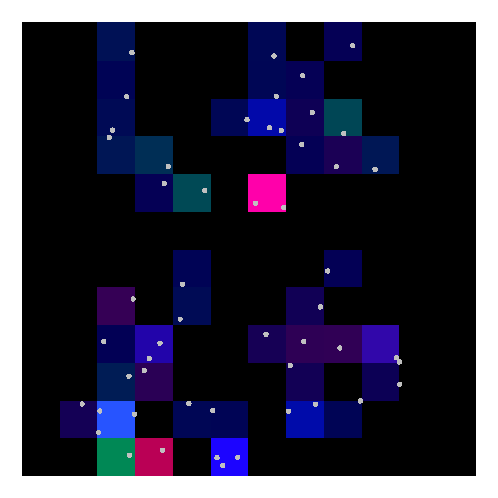
\includegraphics[width=0.49\textwidth]{figures/event_selection/full_image_rect.pdf}
    \end{center}
    \caption{\textbf{Top:} 
             construction of single-jet image from jet constituents. Arrows correspond to individial PF candidates where red arrows are charged, green are neutral and the opacity corresponds to $p_{T}$.
             The red channel measures charged candidate $p_T$ deposition in each pixel, 
             the green channel is neutral charged candidates $p_T$ deposition, 
             and the blue channel is the number of candidates in each pixel (multiplicity). 
             Multiplicity channel is drawn separately so the charged and neutral channels can be seen clearly. Black pixels are lightened to show coloured pixels more clearly.\\
             \textbf{Bottom:} 
             the final image with all the channels together.}
    \label{fig:event_categorisation:jet_image}
\end{figure}



\subsection{Model Design}

The overall structure of the model can be considered to built from three main parts:
\begin{itemize}[leftmargin=.5in,noitemsep]
    \item \textbf{Convolutional section} for learning dijet substructure features from dijet images.
    \item \textbf{Merge section} for processing and integrating engineered kinematic features with learned features from the convolutional section.
    \item \textbf{Main discriminant} fully-connected layers for integrating all information and producing the class logits.
\end{itemize}


The convolutional section consists of a `spread layer' followed by three dense blocks each of which are followed by transition units.

The spread layer is a depthwise convolution layer which produces $N$-many featuremaps for each channel where the filters do not mix the image channels. 
For each channel's associated feature maps half of them have their values evenly permuted in the vertical direction, this corresponds to a rotation by $\pi$ in the polar image.
The function of this layer is to spread out the sparse image into a collection of featuremaps which correspond to simple local spatial configurations of pixels such as radial or angular bands of deposition. 
The interleaved rotations of this layer's output featuremaps allows for the comparison of pixels opposite each other around the jet axis much earlier in the network.  
This layer gives two hyperparameters to the model: the filter size and the number of features per input channel.

The dense blocks construct increasingly higher-level featuremaps, and the transition units will combine feature maps for feature reduction as well as downsampling with average pooling to avoid information loss associated with max pooling mentioned before.  
The structure of each of these parts is tuneable, and therefore gives another twelve hyperparameters to the model: three from each dense block and one from each transition unit. 

The merge section consists of a set of fully-connected layers with the first one after the initial input a different size to the others, this is then concatenated with the output of the convolutional part.
The function of this section is to embed the engineered features in a higher-dimensional space, form them into a vector the same size as the convolutional section output, and then combine them together with the jet structure features. This section has three hyperparameters: the size of the hidden layers, the number of layers, and the size of the first hidden layer relative to the others. 


The main discriminant consists of a sequence of fully-connected layers which take the full vector of concatenated features as input and produce three class logits which correspond to the VBF, ggH, and background process classes. 
These logits are then mapped to class probabilities by a softmax function, the VBF class probability is then used to define tag categories. 

\subsection{Dataset, Training and Loss}
(The loss for training, explain weights as a misclassification cost)
(Cost sensitivity: intra class and inter class costs)
The loss function used is a weighted version of cross entropy where the loss over the minibatch is a weighted mean. For each batch the optimiser will descend the weighted mean of the gradients for each example in the minibatch. The weights are normalised per class so each class has the same total weight, but the shape of their distribution is preserved.  


The optimiser is Adam with nesterov momentum with a learning rate of $0.0001$, slower than the default to ensure smoother filters. 

All of the input features are preprocessed with mean-subtraction and division by their standard deviation. The means and standard deviations are calculated from the training set and these values are applied to the validation and test sets as well as the training set. 
The the training data are augmented by randomly reflecting the images in the $\Delta\eta$ and $\Delta\phi$ directions during training. 

(The regularisation)
The model is regularised with $L_2$ throughout, but with separate values for the different sections. There is also dropout applied to the fully-connected layers during training. 
Dropout is not applied to the convolutional part. 


\subsection{Neural Architecture Search}
Network architecture optimisation

The final model post-opt 

(table of values)

\subsection{Regularization}
Now control the model capactity with regularisation. 

\subsection{Final Model Performance and Categorisation}
The performance of the final model with comparison to the legacy

\subsection{Learned Features Interpretation}
We would like to figure out what sort of features the convolutional section is forming. There are three approaches we will explore here: maximally activating images from the dataset, image occlusion studies, and the production of maximally activating images using stochastic gradient descent (deep dreams).  


\section{Untagged}
If the candidate does not receive a tag it is conisdered for the untagged categories which make a selection diphoton BDT score. These categories mostly consist of gluon fusion events. 


